\documentclass{beamer}

\usepackage[utf8x]{inputenc}
\usepackage[T1]{fontenc}
\usepackage[ngerman]{babel}
\usepackage{helvet}
\usepackage{tikz}
\usepackage{cancel}
\usetikzlibrary{positioning,shapes,calc}

\includeonly{
    metadata,
    content
}

\setbeamertemplate{headline}[default]
\AtBeginSection[]
{
 \begin{frame}
  \frametitle{Fahrplan}
  \tableofcontents[currentsection,hideothersubsections]
 \end{frame}
}


\newcommand{\dcsubject}{Chaos Computer Club M"unchen e.V.}
\newcommand{\dctitle}{MUCCC}
\newcommand{\dcsubtitle}{~}

\newcommand{\dcauthors}{Franz Nord, Franziska Nord}
\newcommand{\dcdate}{\today}

\newcommand{\dcplace}{, M"unchen}

\newcommand{\dckeywords}{Fachpraxis f"ur Datenheilkunde und Hochfrequenztherapie}

\hypersetup{
    pdftitle = {\dctitle},
    pdfsubject = {\dcsubject, \dcdate},
    pdfauthor = {\dcauthors},
    pdfkeywords = {\dckeywords},
    pdfcreator = {pdfTeX with Hyperref},
    pdfproducer = {LaTeX, hyperref},
}



\title{\dctitle}
\author{\dcauthorsshort}
\date{\dcdate}

% Placeholder for the email.tex section, content will be defined there
\newcommand{\emailtext}{}
\newcommand{\emailciphertext}{}
\newlength{\messagewidth}

% For blocks that contain only items
\newenvironment{blit}[1]{%
\begin{block}{#1}
\begin{itemize}
}{%
\end{itemize}
\end{block}
}

\newenvironment{blex}[1]{%
\begin{block}{#1}
\begin{description}
}{%
\end{description}
\end{block}
}

\begin{document}

{%
\setbeamertemplate{background}{}
\begin{frame}[plain]
  \titlepage

  \vfill
  \begin{flushright}
    \href{https://creativecommons.org/licenses/by-sa/4.0/}{\includegraphics[height=3ex]{images/by-sa.png}}
  \end{flushright}
\end{frame}
}

\begin{frame}
\frametitle{Fahrplan}
\tableofcontents[hidesubsections]
\end{frame}

\section{Über den Veranstalter und Cryptopartys}
\begin{frame}{Veranstalter}
\end{frame}

\endinput

\section{Grundlegendes}
\begin{frame}{Warnhinweise}
  \begin{itemize}
    \item 100\% Sicherheit gibt es nicht
    \item Absichern heißt, Angriffe \emph{teurer} zu machen
    \begin{itemize}
    \item Die Kosten für den Angriff\\ müssen den Wert der Daten übersteigen
    \item Ein Angriff darf sich nicht mehr \emph{lohnen}
    \item Problem: Wert wird oft unterschätzt
    \end{itemize}
    \item Was wir hier zeigen, ist ein Anfang
    \begin{itemize}
      \item Hilft dagegen, als ,,Beifang`` zu enden
      \item Gegen gezielte Angriffe -- auch durch Verwechslung -- benötigt es deutlich mehr
    \end{itemize}
%    \item Irren ist menschlich -- auch was die Inhalte der folgenden Folien betrifft :-)
  \end{itemize}
\end{frame}

\begin{frame}{Leitfragen}
  \begin{itemize}
    \item \emph{Was} soll sichergestellt werden?
      \begin{itemize}
        \item Eigene Anonymität
        \item Echtheit des Gegenübers (Authentizität)
        \item Unverfälschtheit der Nachricht (Integrität)
        \item Geheimhaltung der Nachricht (Vertraulichkeit)
        \item \ldots
      \end{itemize}
    \item \emph{Wem} vertraut Ihr?
  \end{itemize}
\end{frame}

\begin{frame}{Vertrauen}
  \begin{block}{Woher weiß man, wem man vertrauen kann?}
  \begin{itemize}
    \item Kurze Antwort: weiß man \emph{nicht}
    \item Lange Antwort
    \begin{itemize}
      \item es gibt Fragen, die man stellen kann\ldots
      \item \ldots\ und es gibt das Bauchgefühl
    \end{itemize}
  \end{itemize}
  \end{block}
\end{frame}

\begin{frame}{Welche Fragen kann man stellen?}
  Beispiel: \emph{Wo} sind meine Daten?
  \begin{itemize}
    \item Auf einem Blatt Papier zuhause in meiner Schublade.
    \item Auf meinem Computer:
    \begin{itemize}
      \item Wie gut ist die Software \emph{überprüfbar},\\ die meine Daten verwaltet?
      \begin{itemize}
        \item Open Source (in menschenlesbarer Form öffentlich):\\gut überprüfbar
        \item Closed Source (menschenlesbare Form geheim):\\quasi nicht überprüfbar
      \end{itemize}
    \end{itemize}
    \item In der Cloud
      %TODO: FSF there is no cloud
      \begin{itemize}
        \item \emph{Wer} betreibt einen Dienst?
        \item Womit \emph{verdient} der Betreiber sein \emph{Geld}?
        \item Wem könnten die Daten \emph{nutzen} oder \emph{schaden}?
        \item Was \emph{lernt} der Betreiber über mich?
      \end{itemize}
  \end{itemize}
\end{frame}

\begin{frame}{Meta- und Nutzdaten}
  \begin{itemize}
    \item Meta-/Verbindungsdaten (``Briefumschlag'')
    \begin{itemize}
      \item Absender, Empfänger, Betreff einer E-Mail
      \item Besuch und Aufenthaltsdauer auf einer Webseite
      \item Wer, wann, wie lange mit wem telefoniert
      \item Aufenthaltsort von Mobiltelefonen: Bewegungsprofil!
    \end{itemize}
    \item Nutz-/Inhaltsdaten (``Brief'')
    \begin{itemize}
      \item E-Mail-Text und -Anhänge
      \item Webseiten-Inhalte
      \item Gesprochene Sprache beim Telefonieren
      \item SMS-Inhalt
    \end{itemize}
  \end{itemize}

Metadaten zu verschlüsseln ist nicht möglich,\\ sie zu verschleiern schwierig.
\end{frame}

\endinput

\section{Passwörter}
\begin{frame}{Passwörter}
  \visible<+->{Wer hat mindestens fünf Online-Accounts?}

  \visible<+->{Wer hat dafür mindestens drei verschiedene Passwörter?}

  \visible<+->{Wer beachtet, Passwörter nur über HTTPS einzugeben?}
\end{frame}

\begin{frame}{Anzahl Passwörter}
  \begin{itemize}
    \item Kundendaten gehen häufig verloren
    \begin{itemize}
      \item Schaden lässt sich begrenzen, wenn Benutzername und Passwort nur bei diesem einen Anbieter passen
    \end{itemize}
    \item Besonders wichtig: E-Mail-Accounts
    \begin{itemize}
      \item Weil ,,Passwort zurücksetzen`` oft via E-Mail
      \item Wer den E-Mail Account übernommen hat,\\ kann dadurch sämtliche Accounts übernehmen
    \end{itemize}
    \item Ideal: Jedes Passwort nur einmal verwenden
    \item Alternative: Passwörter ,,salzen``
    \begin{itemize}
      \item \textit{passwort}.amz für Onlineshop a
      \item \textit{passwort}.zal für Onlineshop z
      \item \textit{anderespasswort} für Mails
    \end{itemize}
  \end{itemize}
\end{frame}

\begin{frame}{Passwort Wiederverwertung}
  \begin{center}
    \includegraphics[height=0.8\textheight]{images/password_reuse_top.png}\\
  \end{center}
  \tiny Bildquelle: Ausschnitt aus \href{http://xkcd.com/792/}{xkcd: Password Reuse / CC BY-NC 2.5}
\end{frame}

\begin{frame}{Sichere Passwörter}
  \begin{block}{Anforderungen}
  \begin{itemize}
    \item Klein- und Großbuchstaben, Zahlen,\\ begrenzt: Sonderzeichen
    \item Wichtiger: Lang genug!
  \end{itemize}
  \end{block}
  \begin{block}{Merkbarkeit}
  \begin{itemize}
    \item Geschichte dazu ausdenken
    \item Melodie und Rhythmus rein bringen
    \begin{itemize}
      \item Gehirn kann sich Melodien besonders leicht merken
      \item Ermöglicht schnelles Eintippen
      \begin{itemize}
        \item Längere Passwörter sind weniger nervig
        \item Passwort mitlesen ist schwieriger
      \end{itemize}
    \end{itemize}
  \end{itemize}
  \end{block}
\end{frame}

\begin{frame}{Passwort Länge vs. Zeichensatz}
  \begin{center}
    \includegraphics[width=0.99\textheight]{images/password_strength.png}\\
  \end{center}
  \tiny Bildquelle: \href{http://xkcd.com/936/}{xkcd: Password Strength / CC BY-NC 2.5}
\end{frame}

\begin{frame}{Passwort-Manager}
  \begin{itemize}
    \item Software zur Verwaltung von Passwörtern
    \item Kann automatisch komplexe Passwörter erzeugen
    \item Datenbank wird mit Master-Passwort verschlüsselt
    \begin{itemize}
      \item Anzahl der zu merkenden Passwörter geringer
    \end{itemize}
    \item Beispiele
    \begin{itemize}
      \item KeePassX (Open Source)
      \item KeePass (Open Source)\\
        \textbf{Achtung:} Unsichere Update-Prüfung vor Version 2.34
    \end{itemize}
  \end{itemize}
  \begin{itemize}
    \item \emph{Wichtige Passwörter trotzdem merken\\oder an einem sicheren Ort aufbewahren!}
  \end{itemize}
\end{frame}

\endinput

\section{Web-Surfen}
\begin{frame}{Tracking}
  \begin{itemize}
    \item Cookies und Co (HTML5 Persistent Local Storage, Flashcookies, \ldots)
    \item Browser-Fingerabdruck
    \item IP-Adresse
  \end{itemize}
  Jede Website und jedes Werbenetzwerk\\kann Personen und Computer (wieder-)erkennen

  \begin{block}{Tools zur Aufklärung}
  \begin{itemize}
    \item \href{https://panopticlick.eff.org/}{EFF: Panopticlick}
    \item \href{http://datenblumen.wired.de/}{Wired: Datenblumen}
  \end{itemize}
  \end{block}
\end{frame}

\begin{frame}{Schutzmaßnahmen -- Level 1}
\framesubtitle{Nur Einstellungen ändern}
  \begin{itemize}
    \item Standardsuchmaschine\\ auf datenschutzfreundliche Anbieter ändern, z.B.
    \begin{itemize}
      \item DuckDuckGo
      \item Startpage
    \end{itemize}
    \item Cookies verbieten, nur selektiv erlauben
    \begin{itemize}
      \item Firefox: about:preferences
    \end{itemize}
    \item Plugins auf ,,Click-to-use`` stellen
    \begin{itemize}
      \item Firefox: about:addons
    \end{itemize}
  \end{itemize}

  Eventuell:
  \begin{itemize}
    \item Blockierung von ,,bösen`` Webseiten abschalten
    \item Statusberichte des Browsers abschalten
  \end{itemize}
\end{frame}

\begin{frame}{Schutzmaßnahmen -- Level 2}
\framesubtitle{Plug-Ins installieren}
  \begin{itemize}
    \item Adblocker --\\ Schadsoftware immer öfter über Werbeanzeigen!
    \begin{itemize}
      \item uBlock origin
      \begin{itemize}
        \item Keine \glqq acceptable adds\grqq\ wie bei Adblock Plus
        \item Blockiert auch andere nervige Dinge außer Werbung
      \end{itemize}
      \item \href{https://www.eff.org/privacybadger}{EFF: Privacy Badger}
      \begin{itemize}
        \item Blockiert anhand von Verhalten, nicht Listen
      \end{itemize}
      %\item TODO: RequestPolicy
    \end{itemize}
    \item NoScript
    \begin{itemize}
      \item Erlaubt gezieltes ein-/ausschalten von Java, JavaScript etc.
    \end{itemize}
    \item EFF: HTTPS-Everywhere
    \begin{itemize}
      \item Nutzt automatisch HTTPS, falls von Seite unterstützt
      \item Benutzt lokale Liste der Seiten, keine Online-Abfrage
    \end{itemize}
    \item RefControl
    \begin{itemize}
      \item HTTP-Referrer = von welcher Seite komme ich
    \end{itemize}
  \end{itemize}
\end{frame}

\begin{frame}{Schutzmaßnahmen -- Level 3}
\framesubtitle{Neue Programme installieren oder benutzen}
  \begin{itemize}
    \item \href{https://www.torproject.org}{Tor Browser Bundle (Freie Software)}
    \begin{itemize}
      \item Anonymisierung des Netzwerkverkehrs\\durch ,,intelligente Umwege''
      \item Fingerabdruck bei allen Tor Browsern identisch
      \item Hohe Sicherheit, aber prinzipbedingt langsamer
    \end{itemize}
    \item \href{https://tails.boum.org}{Tails (Freie Software)}
    \begin{itemize}
      \item Abgesichertes Betriebssystem inkl. Tor
      \item Live System = kann direkt von CD gebootet werden\\ hinterlässt keinerlei Spuren am PC
      % As of 2016-Apr-14, Windows Camouflage has been removed in Tails 2 and newer
      %   https://tails.boum.org/news/windows_camouflage_jessie/index.en.html
      %   https://tails.boum.org/blueprint/update_camouflage_for_jessie/
      %\item Sieht auf Wunsch nach Windows aus
    \end{itemize}
  \end{itemize}
\end{frame}

\endinput

\section{E-Mail}
\begin{frame}{E-Mails: Was soll geschützt werden?}
  E-Mails können
  \begin{itemize}
    \item abgehört
    \item gefälscht
  \end{itemize}
  werden. Deshalb stellen wir vor, wie man
  \begin{itemize}
    \item die Vertraulichkeit (das ,,Briefgeheimnis``) umsetzt
    \\ $\Rightarrow$ Verschlüsselung
    \item die Echtheit des Gegenübers sicherstellt
    \\ $\Rightarrow$ Digitale Signatur
  \end{itemize}
  Außerdem:
  \begin{itemize}
    \item Wie man sicherstellt, dass sein E-Mail Passwort\\ nicht einfach mitgelesen werden kann
  \end{itemize}
\end{frame}

\begin{frame}{E-Mail}{Funktionsweise}
  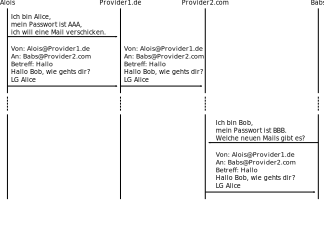
\includegraphics[width=.9\textwidth]{images/maildaten.pdf}
  \scriptsize
  ~\\
  ~\\
\end{frame}

\begin{frame}{E-Mail}{Transportverschlüsselung}
  \includegraphics[width=.9\textwidth]{images/maildaten_trans.pdf}
  \begin{itemize}
    \scriptsize
    \item muss von den Mailanbietern unterstützt werden
    \item Konfiguration des Mailprogramms überprüfen!
  \end{itemize}
\end{frame}

\begin{frame}{E-Mail}{Ende-zu-Ende-Verschlüsselung}
  \includegraphics[width=.9\textwidth]{images/maildaten_e2e.pdf}
  \begin{itemize}
    \scriptsize
    \item unabhängig vom Mailanbieter möglich
    \item verhindert Mitlesen von Mail-\textbf{Nutzdaten}
  \end{itemize}
\end{frame}

\begin{frame}{E-Mail}{Kombination}
  \includegraphics[width=.9\textwidth]{images/maildaten_beides.pdf}
  \scriptsize
  ~\\
  ~\\
\end{frame}
%\begin{frame}{Analogie zur Vertraulichkeit von E-Mails}
%  \begin{itemize}
%    %TODO: überarbeiten
%    \item E-Mails sind ,,Postkarten``
%    \item Transportiert in ,,gläsernen Fahrzeugen``
%    \begin{itemize}
%      \item ,,Autobahnbetreiber`` kann alles mithören
%      \item ,,Post`` kann alles mithören
%    \end{itemize}
%    \item Bei \emph{Transportverschlüsselung} ersetzt die ,,Post``\\ ,,gläserne Fahrzeuge`` durch ,,blickdichte Fahrzeuge``
%    \begin{itemize}
%      \item ,,Autobahnbetreiber`` kann mithören,\\ wann welche ,,Post`` mit welcher ,,Post`` redet\\ aber nicht Passwort, Empfänger, Betreff, etc.
%      \item ,,Post`` kann alles mithören
%    \end{itemize}
%    \item Bei \emph{Ende-zu-Ende-Verschlüsselung} steckt der Absender die ,,Postkarte`` in einen ,,Briefumschlag``
%    \begin{itemize}
%      \item ,,Autobahnbetreiber`` und ,,Post`` können mithören,\\ wann wer mit wem wie viel kommuniziert\\ aber nicht den Inhalt!
%    \end{itemize}
%    \item Unbedingt beides kombinieren!
%  \end{itemize}
%\end{frame}

\begin{frame}{Überprüfung der Echtheit}
Was, wenn A eine Nachricht an B schicken will,\\ aber den öffentlichen Schlüssel von B nicht kennt?\\
\begin{enumerate}
  \item Im ``Telefonbuch'' nach dem Schlüssel suchen
  \item Echtheit mit Hilfe eines \emph{vertrauenswürdigen Dritten} C überprüfen
\end{enumerate}
\begin{center}
  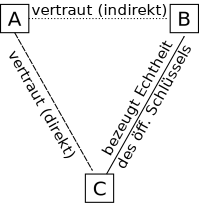
\includegraphics[width=0.5\textheight]{images/vertrauen.pdf}
  %TODO: überarbeiten
\end{center}
\end{frame}

\begin{frame}{Wie stellt man Vertrauen her?}
  \begin{itemize}
    \item S/MIME -- Hierarchischer Vertrauensansatz
    \begin{itemize}
      \item hier nicht behandelt
    \end{itemize}
    \item GnuPG -- Dezentraler Vertrauensansatz
    \begin{itemize}
      \item jeder kann festlegen, wem er vertraut
      \begin{itemize}
        \item er kann die Echtheit eines Schlüssels\\ z.B. bei einem persönlichen Treffen überprüfen
      \end{itemize}
      \item jeder \emph{kann} sein Vertrauensnetz veröffentlichen (Web-of-Trust)
      \begin{itemize}
        \item Vorteil: Man kann ``Freunden von Freunden'' vertrauen
        \item Nachteil: Beziehungen zwischen Menschen öffentlich\\ Aber: Facebook sagt da viel mehr aus
      \end{itemize}
      %\item wird hier behandelt
    \end{itemize}
  \end{itemize}
\end{frame}

\begin{frame}{Welche Software benötigt man?}
  \begin{block}{OpenPGP Backend}
    Macht die eigentliche Ver-/Entschlüsselung \& Signatur

    \vspace{1ex}
    \begin{tabular}{ccc}
      Linux:            & Windows: & Android: \\
      \textit{on-board} & GPG4Win  & APG      \\
    \end{tabular}
  \end{block}
  \begin{block}{Plug-In fürs Mailprogram}
    Grafische Oberfläche, leichtere Schlüsselverwaltung, etc.

    \vspace{1ex}
    \begin{tabular}{ccc}
      Thunderbird: & Outlook: & K9-Mail: \\
      Enigmail     & GPG4Win  & APG      \\
    \end{tabular}
  \end{block}
\end{frame}

\endinput

\section{Messenger}
\begin{frame}{Motivation}
\begin{itemize}
\item Komfortabel, auf Smartphone einfach nutzbar
\item Wird im privaten Umfeld meist häufiger eingesetzt\\ als E-Mail
\end{itemize}

\pause
\begin{block}{Bestandsaufnahme}
Wer benutzt
\begin{itemize}
\item<+-> WhatsApp
\item<+-> Telegram
\item<+-> Threema
\item<+-> Signal
\item<+-> Jabber
\end{itemize}
\end{block}
\end{frame}

\begin{frame}{Überblick}
  \begin{itemize}
    \item Geschlossene Systeme: WhatsApp \& Co
      \begin{itemize}
        \item App-Entwickler\\
          ist Dienstanbieter\\
          und Herr über die ``technische Sprache'' (das Protokoll)
        \item Auswahl eines Dienstes\\bestimmt erreichbaren Personenkreis
        \item meist Closed Source
      \end{itemize}
    \item Offene Systeme wie Jabber/XMPP
      \begin{itemize}
        \item App-Entwickler, Dienstanbieter und Protokoll-Standardisierer sind unterschiedliche Personen
        \item App und Anbieter frei wählbar
        \item meist Open Source
      \end{itemize}
  \end{itemize}
\end{frame}

\setbeamersize{description width=1em}
\begin{frame}[t] % align on top so EFF scorecard does not move
\frametitle{Vor- und Nachteile}

\only<+>{
\begin{blex}{WhatsApp}
\item[+] Nutzdaten werden verschlüsselt
\item[+] Android: Verwendbar ohne Google Play
\item[-] Closed Source
\item[-] Anbieter erhält eine Kopie des vollständigen Telefonbuchs\\
  (nicht nur WhatsApp-Kontakte)
\end{blex}

\textbf{Tipp:} Wer sein Telefonbuch nicht freigeben will,\\
  kann den Zugriff darauf verweigern\\
  (Android: ab Version 6).

Der Nutzungskomfort ist dadurch eingeschränkt.
}

\only<+>{
\begin{blex}{Signal}
\item[+] Nutzdaten werden verschlüsselt
\item[-] Android: Nicht verwendbar ohne Google Play
\item[-] Anbieter erhält eine Kopie des vollständigen Telefonbuchs\\
  (nicht nur Signal-Kontakte)
\end{blex}}

\only<+>{
\begin{blex}{Telegram}
\item[+] \glqq Verschlüsselte Chats\grqq\ möglich
\item[-] Anbieter erhält eine Kopie des vollständigen Telefonbuchs
\item[-] Verschlüsselung standardmäßig nicht aktiv
\item[-] \glqq Normale Chats\grqq\ werden im Klartext auf den Servern gespeichert
\end{blex}}

\only<+>{
\begin{blex}{Threema}
\item[+] Chats verschlüsselt
\item[+] komfortabler Schlüsselaustausch über QR-Code
\item[+] Synchronisation des Telefonbuchs ist optional
\item[-] Closed Source
\item    kostenpflichtig
\end{blex}}


\only<+>{
\begin{blex}{Jabber/XMPP}
\item[+] Offenes System: Anbieter und App frei wählbar
\item[+] Verschlüsselung möglich (OTR oder OMEMO)
\item[+] keine Telefonbuch-Synchronisation vorgesehen
\item[-] Crypto nicht ganz so nutzerfreundlich\\wie bei kommerziellen Anbietern\\(aber dafür sind wir ja alle hier :-)
\end{blex}
\begin{itemize}
  \item    Apps: Conversations, pidgin, gajim, \ldots 
  \item    Anbieter: Unis, Hackerspaces, CCC, jabber.org, \ldots
\end{itemize}

}
\end{frame}

\begin{frame}{Zusammenfassung}
  \begin{itemize}
    \item Wer auf bestimmten Messenger nicht verzichten kann:\\Zugriff auf Kontakte verbieten!
    \item Weitere Infos: EFF Secure Messaging Scorecard\\ {\url{https://www.eff.org/secure-messaging-scorecard}}\\
      (gerade in Überarbeitung, alte Version noch verlinkt)
  \end{itemize}
  
\end{frame}

\section{Fragen, Feedback}
\begin{frame}{Fragen, Feedback, ...}
  \begin{itemize}
    \item{Her damit!}
    \item{Fragen an alle Helfer (bitte gebt Euch zu erkennen :-)}
    \item{Links}
      \begin{itemize}
        \item \url{https://www.prism-break.org}
        \item \url{https://muc.pads.ccc.de/cryptoparty}
        \item \url{https://github.com/muccc/cryptoparty-intro/tree/flo-ccc-fiff-mzm}
      \end{itemize}
  \end{itemize}
\end{frame}

\endinput


\end{document}
